\section{Behavior} \label{sc:behavoir}
In the following section, the behavior of each class will be examined. A deeper understanding of these behaviours will be achieved through state chart diagrams.
\\\\

\large{\textbf{Asset}}
\begin{figure}[H]
    \centering
    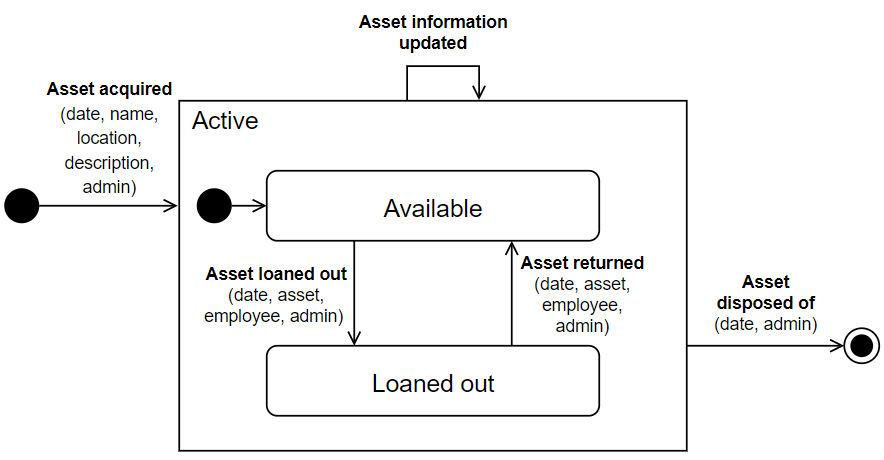
\includegraphics[width=1\textwidth]{figures/StateCharts/Asset_state_chart.png}
    \caption{State chart diagram for the \textbf{Asset} class}
    \label{fig:asset_statechart}
\end{figure}

An object of the \textit{Asset} class is created when an asset is acquired. At first, its state is \textbf{Available}, and when the asset is loaned out to an employee, it changes state to \textbf{Loaned out}. From any of these two states, the asset can be disposed of and removed from the problem domain. Being loaned out will, in the system, simply consist of the asset being tagged with an employee, and the return of the asset will be removing this relation. The information on the asset, not including the tags attached to it, can be updated at all times during its life cycle in the system, and can occur multiple times.
\\\\

\large{\textbf{Employee}}
\begin{figure}[H]
    \centering
    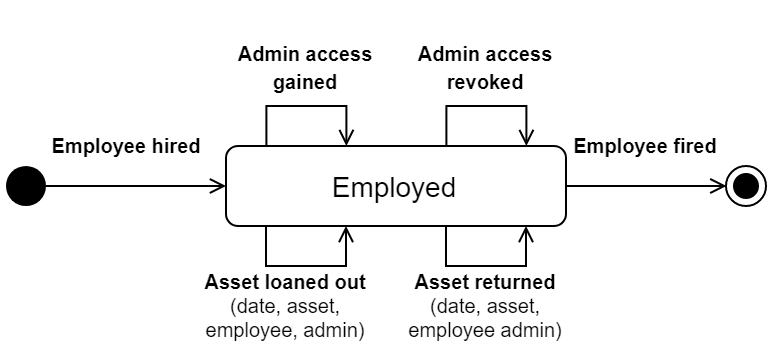
\includegraphics[width=0.8\textwidth]{figures/StateCharts/StateChart_Employee.png}
    \caption{State chart diagram for the \textbf{Employee} class}
    \label{fig:employee_statechart}
\end{figure}

An \textit{Employee} object is created when a person is hired at the zoo and gains the status employed. An employee can be granted admin access, which can later be revoked. An employee can also borrow an asset and return it later. The employee object ceases to exist when the person is fired. The event of returning an asset can only happen when the employee has borrowed the given asset, but an employee can borrow multiple assets at a time, hence both events are iterations.\\
The employee can be granted admin access multiple times during the employment but of course, the access can only be revoked after the access has been granted. Both things can happen multiple times and are therefore iterations. These two events also mark the initialization and end of an admin.
\\\\

\large{\textbf{Admin}}
\begin{figure}[H]
    \centering
    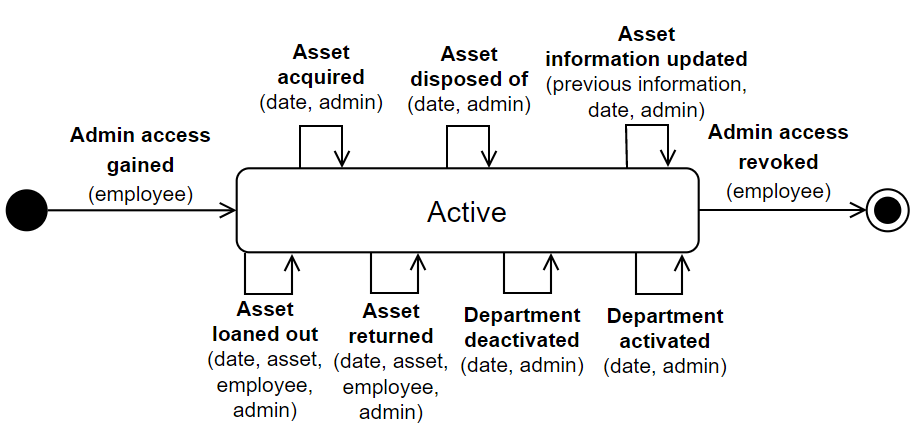
\includegraphics[width=0.8\textwidth]{figures/StateCharts/Admin_state_chart.png}
    \caption{State chart diagram for the \textbf{Admin} class}
    \label{fig:admin_statechart}
\end{figure}

The \textit{Admin} object is created when an employee is granted admin access. As an admin, the employee is responsible for loaning out assets to other employees and receiving the assets when they are returned. The admin will also be responsible for adding tags, assets, activating departments, and maintaining these elements by updating and removing them. The admin object is terminated when the employee's admin access is revoked.
\\\\

\large{\textbf{Tag}}
\begin{figure}[H]
    \centering
    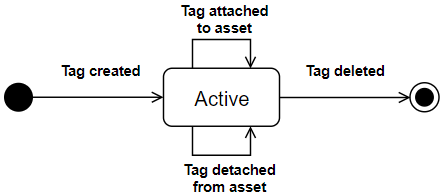
\includegraphics[width=0.6\textwidth]{figures/StateCharts/Tag_state_chart.png}
    \caption{State chart diagram for the \textbf{Tag} class}
    \label{fig:loan_statechart}
\end{figure}

An object of the \textit{Tag} class is created by an admin and can be attached to and detached from assets multiple times during its life cycle. The tag is terminated when an admin deletes it from the system.
\par

With the behaviours of the classes described, the problem domain has been analysed. The following section will sum up the results of the analysis.

% \large{\textbf{Loan}}
% \begin{figure}[H]
%     \centering
%     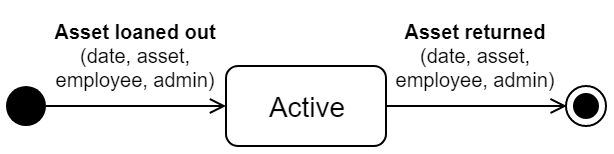
\includegraphics[width=0.8\textwidth]{figures/StateChart_Loan.png}
%     \caption{State chart diagram for the \textbf{Loan} class}
%     \label{fig:loan_statechart}
% \end{figure}

% A \textbf{Loan} object is created when an asset is loaned out and seizes to exist when the asset is returned.
% \newline\par
% With the behaviours of the classes described, the problem domain has been analysed. The following section will sum up the results of the analysis.